%Praesentationsmodus
\documentclass[t,aspectratio=169,divpsnames]{beamer}
%Die Beameroption aspectratio legt das verwendete Seitenverhaeltnis fest
%aspectratio=169	16:9 Seitenverhaeltnis
%aspectratio=1610	16:10 Seitenverhaeltnis
%aspectratio=43		4:3 Seitenverhaeltnis
%Die Beameroption envcountsect nummeriert Umgebungen wie theorem pro section durch.
%Die Beameroption divpsnames wird an das xcolor Paket durchgereicht.

%Handout-Generierung mit Foliennotizen (statt obiger Zeile für den Präsentationsmodus verwenden)
%\documentclass[t,handout,aspectratio=169]{beamer}
%\setbeameroption{show notes}

\usepackage[utf8]{inputenc}

% Deutsch
\usepackage[ngerman]{babel} 
\usepackage{bibgerm}

% Englisch
%\usepackage[english]{babel}

\input{templatesetup}
\usepackage{listings}
\lstset
{
	basicstyle=\ttfamily, 
	keywordstyle=\color{blue}\bfseries\ttfamily,
	identifierstyle=\ttfamily, 
	stringstyle=\ttfamily,
	commentstyle=\color{ForestGreen},
	showstringspaces=false,
	framexleftmargin=7mm, 
	breaklines=true,
	tabsize=3,
	showtabs=false,
	frame=single, 
	rulesepcolor=\color{blue},
	numbers=left,
	linewidth=146mm,
	xleftmargin=8mm,
	language={C++},
}

% Stil des Literaturverzeichnisses
\bibliographystyle{geralpha}
%\bibliographystyle{alpha}
%\bibliographystyle{abstract}

%Bitte ausfuellen:
\title{Kolloquiumsvortrag}
\subtitle{Entwicklung eines 2D Charakter-Animationssystemes für automatische Laufbewegungen}
\author{Daniel Track}
\institute{Hochschule Trier}
\date{03.11.2020}
\subject{Thema für PDF-Metadaten (optional)}

%Inhaltsverzeichnisses bis auf subsubsection-Ebene:
%\setcounter{tocdepth}{3}

%Aktivieren, um am Anfang jeder Section ein Inhaltsverzeichnis zur Section anzuzeigen
%\AtBeginSection[]
%{
%\begin{frame}<beamer>
%\frametitle{Agenda}
%\tableofcontents[currentsection,hideothersubsections,sectionstyle=show/hide,subsubsectionstyle=show/show]
%\end{frame}
%}

%Aktivieren, um alles Schritt-fuer-Schritt einzublenden
%\beamerdefaultoverlayspecification{<+->}

\begin{document}

\begin{frame}
    \titlepage
\end{frame}

\begin{frame}
    \frametitle{Agenda}
    \tableofcontents
    %\tableofcontents[hideallsubsections] % Subsections ausblenden
    %\tableofcontents[pausesections] %Sections Schritt-fuer-Schritt einblenden
\end{frame}

\section{Einleitung}
\begin{frame}{Einleitung}{Motivation}
    \begin{itemize}
        \item Gängige 2D-Animationssysteme benötigen oft sehr viele Sprites % Gibt natürlich Ausnahmen/andere Systeme 
        \item Nicht einfach skalierbar für hohe Framerates ($>$ 60 fps)
        \item Skelettbasierte 3D-Animation hat diese Probleme nicht
        \item Außerdem flexibler, da Runtime-Daten in die Animation mit einbezogen werden können
    \end{itemize}

    $\Rightarrow$ Warum nicht das 3D-System auf 2D-Charaktere übertragen?
\end{frame}

\begin{frame}{Einleitung}{Zielsetzung}
    \begin{itemize}
        \item Generierung von glaubhaften Laufanimationen aus einem einzelnen Sprite, gepaart mit einem Skelett
        \item Bewegung über verschieden hohe Untergründe durch Einbeziehung von Laufzeitdaten
        \item Responsive Steuerung
              \begin{itemize}
                  \item Schnelle Reaktion auf Inputs
                  \item Laufgeschwindigkeit mit Control-Stick präzise regulierbar
              \end{itemize}
        \item Anpassbarkeit des Animationsverhaltens
    \end{itemize}
\end{frame}


\section{Forschungsstand}
\begin{frame}{Forschungsstand}{3D-Animation}
    \begin{itemize}
        \item Viele Arbeiten zur 3D-Animation mit Skeletten vorhanden % Rig, Keyposes, Splines sind ein gängiges Verfahren, hier nicht weiter erläutert
        \item Die Arbeit orientiert sich an \cite{johansen2009automated}
              \begin{itemize}
                  \item Kombination aus prozeduralen Verfahren mit zwei Beispielanimationen (Walk und Strafe)
                  \item Synthese von neuen Animationsabläufen aus diesen beiden Beispielen
                  \item Inverse Kinematics zur Anpassung an den Untergrund
              \end{itemize}
        \item Dieser Ansatz wurde übernommen und auf die 2D-Animation übertragen
    \end{itemize}
\end{frame}

\begin{frame}{Forschungsstand}{Skelettale 2D-Animation}
    \begin{itemize}
        \item Literatur beschäftigt sich meist nicht mit Videospielen % Dadurch anderer Fokus als hier
              \begin{itemize}
                  \item Fokus auf Offline-Rendering
                  \item Keine Interaktivität vorgesehen
                  \item Resultate können überprüft werden, bevor das Publikum sie sieht
              \end{itemize}
        \item Teilweise Verwendung von 3D-Modelle zur Erstellung von 2D-Animationen (z.B. \cite{pangesti2019analysis}) % Macht Erstellungsprozess komplizierter
              \begin{itemize}
                  \item Eventuell bessere Animationen durch Verdeckung von Körperteilen möglich
                  \item Macht aber Erstellung der Charaktermodelle komplizierter
              \end{itemize}
        \item Einige Spiele scheinen aber solche Verfahren zu verwenden (z.B. Rain World, QWOP)
    \end{itemize}
\end{frame}

\section{Implementierung}
\begin{frame}{Implementierung}{Animationsprozess}
    \begin{itemize}
        \item Charakter hat drei Beispielanimationen, aus denen die neuen Animationen generiert werden (Idle, Walk, Run)
        \item Animationen definieren Splines für Hände, Füße und Becken
        \item Input des Control-Sticks bestimmt Schrittweite und Interpolationsfaktor zwischen Walk- und Run-Splines
        \item Position des Charakters wird durch Becken festgelegt
        \item Zusätzlich lehnt sich der Charakter mit steigender Geschwindigkeit in die Bewegungsrichtung
    \end{itemize}
\end{frame}

\begin{frame}{Implementierung}{Aktivitätsdiagramm Animator}
    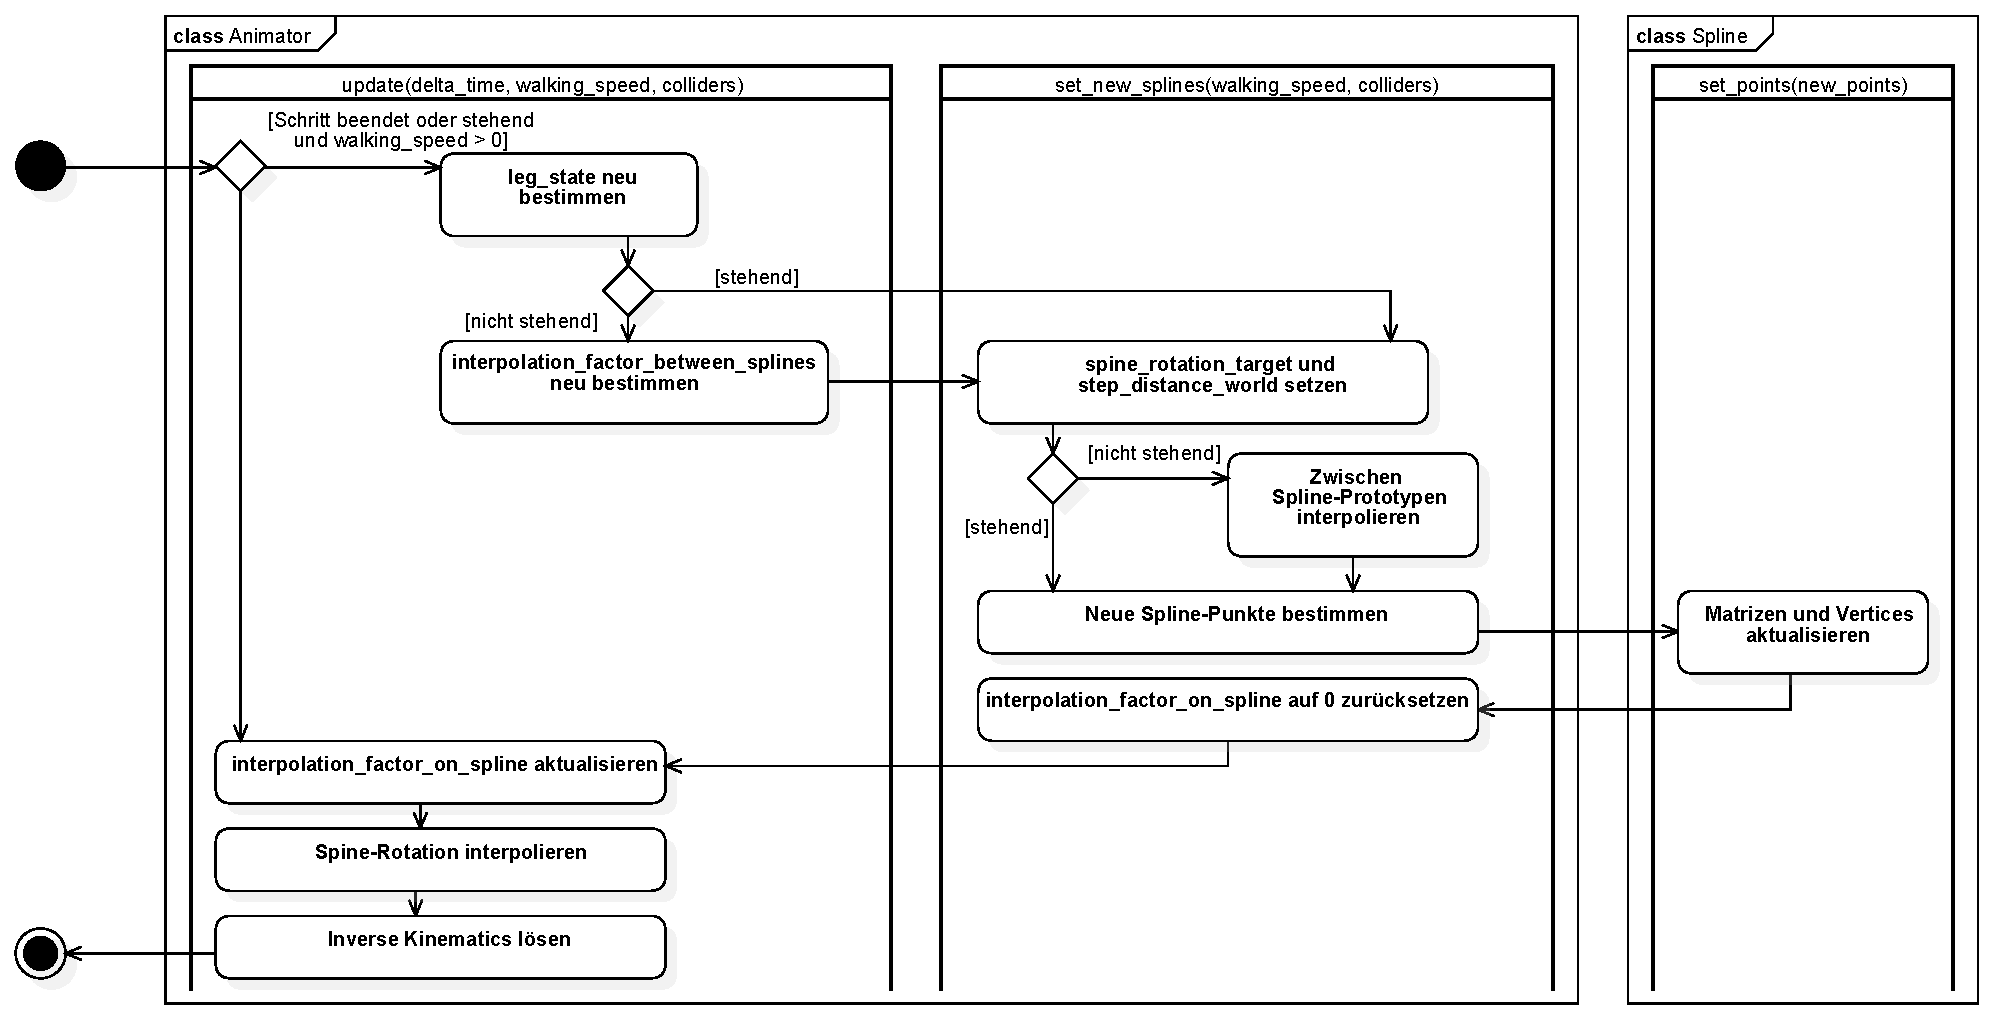
\includegraphics[height=\textheight]{AnimatorActivity_presentation.pdf}
\end{frame}


\section{Ergebnisse}
\begin{frame}{Ergebnisse}{Live Demonstration}
    \begin{center}
        \huge{(Demonstration des Programms)}
    \end{center}
\end{frame}

\begin{frame}{Ergebnisse}{Möglichkeiten zur Verbesserung und Erweiterung}
    \begin{itemize}
        \item Collision-Detection für gesamte Splines (nicht nur Start- und Endpunkt)
        \item Eventuell kombiniert mit Einführung eines dritten Punktes für die Splines, was auch die Customization verbessern sollte
        \item Komplexerer Algorithmus zur Suche von Zielpositionen für Füße, sodass mehr Variation in Leveln möglich ist
              \begin{itemize}
                  \item Schräge Oberflächen
                  \item Mehrere ''Ebenen"
              \end{itemize}
    \end{itemize}
\end{frame}

\section*{Schluss}
\begin{frame}
    \begin{center}
        \huge{Vielen Dank für Ihre Aufmerksamkeit!}
    \end{center}
    \begin{center}
        \Huge{Fragen?}
    \end{center}
\end{frame}

\begin{frame}[allowframebreaks]{\bibname}
    \bibliography{literatur}     %BibTeX-Datei literatur.bib
\end{frame}


\end{document}
